% Options for packages loaded elsewhere
\PassOptionsToPackage{unicode}{hyperref}
\PassOptionsToPackage{hyphens}{url}
\PassOptionsToPackage{dvipsnames,svgnames,x11names}{xcolor}
%
\documentclass[
  letterpaper,
  DIV=11,
  numbers=noendperiod]{scrartcl}

\usepackage{amsmath,amssymb}
\usepackage{iftex}
\ifPDFTeX
  \usepackage[T1]{fontenc}
  \usepackage[utf8]{inputenc}
  \usepackage{textcomp} % provide euro and other symbols
\else % if luatex or xetex
  \usepackage{unicode-math}
  \defaultfontfeatures{Scale=MatchLowercase}
  \defaultfontfeatures[\rmfamily]{Ligatures=TeX,Scale=1}
\fi
\usepackage{lmodern}
\ifPDFTeX\else  
    % xetex/luatex font selection
\fi
% Use upquote if available, for straight quotes in verbatim environments
\IfFileExists{upquote.sty}{\usepackage{upquote}}{}
\IfFileExists{microtype.sty}{% use microtype if available
  \usepackage[]{microtype}
  \UseMicrotypeSet[protrusion]{basicmath} % disable protrusion for tt fonts
}{}
\makeatletter
\@ifundefined{KOMAClassName}{% if non-KOMA class
  \IfFileExists{parskip.sty}{%
    \usepackage{parskip}
  }{% else
    \setlength{\parindent}{0pt}
    \setlength{\parskip}{6pt plus 2pt minus 1pt}}
}{% if KOMA class
  \KOMAoptions{parskip=half}}
\makeatother
\usepackage{xcolor}
\setlength{\emergencystretch}{3em} % prevent overfull lines
\setcounter{secnumdepth}{-\maxdimen} % remove section numbering
% Make \paragraph and \subparagraph free-standing
\makeatletter
\ifx\paragraph\undefined\else
  \let\oldparagraph\paragraph
  \renewcommand{\paragraph}{
    \@ifstar
      \xxxParagraphStar
      \xxxParagraphNoStar
  }
  \newcommand{\xxxParagraphStar}[1]{\oldparagraph*{#1}\mbox{}}
  \newcommand{\xxxParagraphNoStar}[1]{\oldparagraph{#1}\mbox{}}
\fi
\ifx\subparagraph\undefined\else
  \let\oldsubparagraph\subparagraph
  \renewcommand{\subparagraph}{
    \@ifstar
      \xxxSubParagraphStar
      \xxxSubParagraphNoStar
  }
  \newcommand{\xxxSubParagraphStar}[1]{\oldsubparagraph*{#1}\mbox{}}
  \newcommand{\xxxSubParagraphNoStar}[1]{\oldsubparagraph{#1}\mbox{}}
\fi
\makeatother

\usepackage{color}
\usepackage{fancyvrb}
\newcommand{\VerbBar}{|}
\newcommand{\VERB}{\Verb[commandchars=\\\{\}]}
\DefineVerbatimEnvironment{Highlighting}{Verbatim}{commandchars=\\\{\}}
% Add ',fontsize=\small' for more characters per line
\usepackage{framed}
\definecolor{shadecolor}{RGB}{241,243,245}
\newenvironment{Shaded}{\begin{snugshade}}{\end{snugshade}}
\newcommand{\AlertTok}[1]{\textcolor[rgb]{0.68,0.00,0.00}{#1}}
\newcommand{\AnnotationTok}[1]{\textcolor[rgb]{0.37,0.37,0.37}{#1}}
\newcommand{\AttributeTok}[1]{\textcolor[rgb]{0.40,0.45,0.13}{#1}}
\newcommand{\BaseNTok}[1]{\textcolor[rgb]{0.68,0.00,0.00}{#1}}
\newcommand{\BuiltInTok}[1]{\textcolor[rgb]{0.00,0.23,0.31}{#1}}
\newcommand{\CharTok}[1]{\textcolor[rgb]{0.13,0.47,0.30}{#1}}
\newcommand{\CommentTok}[1]{\textcolor[rgb]{0.37,0.37,0.37}{#1}}
\newcommand{\CommentVarTok}[1]{\textcolor[rgb]{0.37,0.37,0.37}{\textit{#1}}}
\newcommand{\ConstantTok}[1]{\textcolor[rgb]{0.56,0.35,0.01}{#1}}
\newcommand{\ControlFlowTok}[1]{\textcolor[rgb]{0.00,0.23,0.31}{\textbf{#1}}}
\newcommand{\DataTypeTok}[1]{\textcolor[rgb]{0.68,0.00,0.00}{#1}}
\newcommand{\DecValTok}[1]{\textcolor[rgb]{0.68,0.00,0.00}{#1}}
\newcommand{\DocumentationTok}[1]{\textcolor[rgb]{0.37,0.37,0.37}{\textit{#1}}}
\newcommand{\ErrorTok}[1]{\textcolor[rgb]{0.68,0.00,0.00}{#1}}
\newcommand{\ExtensionTok}[1]{\textcolor[rgb]{0.00,0.23,0.31}{#1}}
\newcommand{\FloatTok}[1]{\textcolor[rgb]{0.68,0.00,0.00}{#1}}
\newcommand{\FunctionTok}[1]{\textcolor[rgb]{0.28,0.35,0.67}{#1}}
\newcommand{\ImportTok}[1]{\textcolor[rgb]{0.00,0.46,0.62}{#1}}
\newcommand{\InformationTok}[1]{\textcolor[rgb]{0.37,0.37,0.37}{#1}}
\newcommand{\KeywordTok}[1]{\textcolor[rgb]{0.00,0.23,0.31}{\textbf{#1}}}
\newcommand{\NormalTok}[1]{\textcolor[rgb]{0.00,0.23,0.31}{#1}}
\newcommand{\OperatorTok}[1]{\textcolor[rgb]{0.37,0.37,0.37}{#1}}
\newcommand{\OtherTok}[1]{\textcolor[rgb]{0.00,0.23,0.31}{#1}}
\newcommand{\PreprocessorTok}[1]{\textcolor[rgb]{0.68,0.00,0.00}{#1}}
\newcommand{\RegionMarkerTok}[1]{\textcolor[rgb]{0.00,0.23,0.31}{#1}}
\newcommand{\SpecialCharTok}[1]{\textcolor[rgb]{0.37,0.37,0.37}{#1}}
\newcommand{\SpecialStringTok}[1]{\textcolor[rgb]{0.13,0.47,0.30}{#1}}
\newcommand{\StringTok}[1]{\textcolor[rgb]{0.13,0.47,0.30}{#1}}
\newcommand{\VariableTok}[1]{\textcolor[rgb]{0.07,0.07,0.07}{#1}}
\newcommand{\VerbatimStringTok}[1]{\textcolor[rgb]{0.13,0.47,0.30}{#1}}
\newcommand{\WarningTok}[1]{\textcolor[rgb]{0.37,0.37,0.37}{\textit{#1}}}

\providecommand{\tightlist}{%
  \setlength{\itemsep}{0pt}\setlength{\parskip}{0pt}}\usepackage{longtable,booktabs,array}
\usepackage{calc} % for calculating minipage widths
% Correct order of tables after \paragraph or \subparagraph
\usepackage{etoolbox}
\makeatletter
\patchcmd\longtable{\par}{\if@noskipsec\mbox{}\fi\par}{}{}
\makeatother
% Allow footnotes in longtable head/foot
\IfFileExists{footnotehyper.sty}{\usepackage{footnotehyper}}{\usepackage{footnote}}
\makesavenoteenv{longtable}
\usepackage{graphicx}
\makeatletter
\newsavebox\pandoc@box
\newcommand*\pandocbounded[1]{% scales image to fit in text height/width
  \sbox\pandoc@box{#1}%
  \Gscale@div\@tempa{\textheight}{\dimexpr\ht\pandoc@box+\dp\pandoc@box\relax}%
  \Gscale@div\@tempb{\linewidth}{\wd\pandoc@box}%
  \ifdim\@tempb\p@<\@tempa\p@\let\@tempa\@tempb\fi% select the smaller of both
  \ifdim\@tempa\p@<\p@\scalebox{\@tempa}{\usebox\pandoc@box}%
  \else\usebox{\pandoc@box}%
  \fi%
}
% Set default figure placement to htbp
\def\fps@figure{htbp}
\makeatother
% definitions for citeproc citations
\NewDocumentCommand\citeproctext{}{}
\NewDocumentCommand\citeproc{mm}{%
  \begingroup\def\citeproctext{#2}\cite{#1}\endgroup}
\makeatletter
 % allow citations to break across lines
 \let\@cite@ofmt\@firstofone
 % avoid brackets around text for \cite:
 \def\@biblabel#1{}
 \def\@cite#1#2{{#1\if@tempswa , #2\fi}}
\makeatother
\newlength{\cslhangindent}
\setlength{\cslhangindent}{1.5em}
\newlength{\csllabelwidth}
\setlength{\csllabelwidth}{3em}
\newenvironment{CSLReferences}[2] % #1 hanging-indent, #2 entry-spacing
 {\begin{list}{}{%
  \setlength{\itemindent}{0pt}
  \setlength{\leftmargin}{0pt}
  \setlength{\parsep}{0pt}
  % turn on hanging indent if param 1 is 1
  \ifodd #1
   \setlength{\leftmargin}{\cslhangindent}
   \setlength{\itemindent}{-1\cslhangindent}
  \fi
  % set entry spacing
  \setlength{\itemsep}{#2\baselineskip}}}
 {\end{list}}
\usepackage{calc}
\newcommand{\CSLBlock}[1]{\hfill\break\parbox[t]{\linewidth}{\strut\ignorespaces#1\strut}}
\newcommand{\CSLLeftMargin}[1]{\parbox[t]{\csllabelwidth}{\strut#1\strut}}
\newcommand{\CSLRightInline}[1]{\parbox[t]{\linewidth - \csllabelwidth}{\strut#1\strut}}
\newcommand{\CSLIndent}[1]{\hspace{\cslhangindent}#1}

\KOMAoption{captions}{tableheading}
\makeatletter
\@ifpackageloaded{tcolorbox}{}{\usepackage[skins,breakable]{tcolorbox}}
\@ifpackageloaded{fontawesome5}{}{\usepackage{fontawesome5}}
\definecolor{quarto-callout-color}{HTML}{909090}
\definecolor{quarto-callout-note-color}{HTML}{0758E5}
\definecolor{quarto-callout-important-color}{HTML}{CC1914}
\definecolor{quarto-callout-warning-color}{HTML}{EB9113}
\definecolor{quarto-callout-tip-color}{HTML}{00A047}
\definecolor{quarto-callout-caution-color}{HTML}{FC5300}
\definecolor{quarto-callout-color-frame}{HTML}{acacac}
\definecolor{quarto-callout-note-color-frame}{HTML}{4582ec}
\definecolor{quarto-callout-important-color-frame}{HTML}{d9534f}
\definecolor{quarto-callout-warning-color-frame}{HTML}{f0ad4e}
\definecolor{quarto-callout-tip-color-frame}{HTML}{02b875}
\definecolor{quarto-callout-caution-color-frame}{HTML}{fd7e14}
\makeatother
\makeatletter
\@ifpackageloaded{caption}{}{\usepackage{caption}}
\AtBeginDocument{%
\ifdefined\contentsname
  \renewcommand*\contentsname{Table of contents}
\else
  \newcommand\contentsname{Table of contents}
\fi
\ifdefined\listfigurename
  \renewcommand*\listfigurename{List of Figures}
\else
  \newcommand\listfigurename{List of Figures}
\fi
\ifdefined\listtablename
  \renewcommand*\listtablename{List of Tables}
\else
  \newcommand\listtablename{List of Tables}
\fi
\ifdefined\figurename
  \renewcommand*\figurename{Figure}
\else
  \newcommand\figurename{Figure}
\fi
\ifdefined\tablename
  \renewcommand*\tablename{Table}
\else
  \newcommand\tablename{Table}
\fi
}
\@ifpackageloaded{float}{}{\usepackage{float}}
\floatstyle{ruled}
\@ifundefined{c@chapter}{\newfloat{codelisting}{h}{lop}}{\newfloat{codelisting}{h}{lop}[chapter]}
\floatname{codelisting}{Listing}
\newcommand*\listoflistings{\listof{codelisting}{List of Listings}}
\makeatother
\makeatletter
\makeatother
\makeatletter
\@ifpackageloaded{caption}{}{\usepackage{caption}}
\@ifpackageloaded{subcaption}{}{\usepackage{subcaption}}
\makeatother

\usepackage{bookmark}

\IfFileExists{xurl.sty}{\usepackage{xurl}}{} % add URL line breaks if available
\urlstyle{same} % disable monospaced font for URLs
\hypersetup{
  pdftitle={Spatial Pattern of Electric Vehicle Population in State of Washington},
  colorlinks=true,
  linkcolor={blue},
  filecolor={Maroon},
  citecolor={Blue},
  urlcolor={Blue},
  pdfcreator={LaTeX via pandoc}}


\title{Spatial Pattern of Electric Vehicle Population in State of
Washington}
\usepackage{etoolbox}
\makeatletter
\providecommand{\subtitle}[1]{% add subtitle to \maketitle
  \apptocmd{\@title}{\par {\large #1 \par}}{}{}
}
\makeatother
\subtitle{DSAN 6750 / PPOL 6805: GIS for Spatial Data Science}
\author{Christy Hsu}
\date{}

\begin{document}
\maketitle


\subsection{Intro}\label{intro}

This project attempts to provide insights into the spatial pattern of EV
adoptionusing approaches from spatial data science.

The Electric Vehicle Population Data provided by Washington State
Department of Licensing is the main dataset used in this
project.(\citeproc{ref-ElectricVehiclePopulation}{{``Electric {Vehicle
Population Data} {\textbar} {Data}.{WA} {\textbar} {State} of
{Washington}''} 2024})

Two main sections in this project covers:

Initial Evidence

\begin{itemize}
\tightlist
\item
  Visualization
\item
  Global Moran's I
\item
  Local Moran's I
\end{itemize}

Hypothesis Testing

\begin{itemize}
\tightlist
\item
  Intensity Function
\item
  Relative Intensity Surface
\item
  Monte Carlo Simulation
\end{itemize}

\subsubsection{Set up}\label{set-up}

\paragraph{packages}\label{packages}

\textsubscript{Source:
\href{https://h-christy.github.io/24-manuscript/index.qmd.html}{Article
Notebook}}

\paragraph{loading files}\label{loading-files}

\textsubscript{Source:
\href{https://h-christy.github.io/24-manuscript/index.qmd.html}{Article
Notebook}}

\begin{verbatim}
Reading layer `ev1203' from data source 
  `/Users/toyuan/24-manuscript/data/ev1203.gpkg' using driver `GPKG'
Simple feature collection with 208002 features and 25 fields
Geometry type: POINT
Dimension:     XY
Bounding box:  xmin: -124.6274 ymin: 45.596 xmax: -117.0455 ymax: 48.99205
Geodetic CRS:  WGS 84
\end{verbatim}

\begin{verbatim}
Reading layer `wa_poly' from data source 
  `/Users/toyuan/24-manuscript/data/wa_poly.gpkg' using driver `GPKG'
Simple feature collection with 1 feature and 14 fields
Geometry type: POLYGON
Dimension:     XY
Bounding box:  xmin: -124.849 ymin: 45.54354 xmax: -116.9161 ymax: 49.00244
Geodetic CRS:  NAD83
\end{verbatim}

\begin{verbatim}
Reading layer `urban_shape' from data source 
  `/Users/toyuan/24-manuscript/data/urban_shape.gpkg' using driver `GPKG'
Simple feature collection with 56 features and 12 fields
Geometry type: MULTIPOLYGON
Dimension:     XY
Bounding box:  xmin: -124.1802 ymin: 45.78668 xmax: -117.0418 ymax: 49.0021
Geodetic CRS:  WGS 84
\end{verbatim}

\begin{verbatim}
Reading layer `stations' from data source 
  `/Users/toyuan/24-manuscript/data/stations.gpkg' using driver `GPKG'
Simple feature collection with 2800 features and 1 field
Geometry type: POINT
Dimension:     XY
Bounding box:  xmin: -124.6629 ymin: 25.91606 xmax: -73.98274 ymax: 48.99526
Geodetic CRS:  WGS 84
\end{verbatim}

\begin{verbatim}
Reading layer `ct1202' from data source 
  `/Users/toyuan/24-manuscript/data/ct1202.gpkg' using driver `GPKG'
Simple feature collection with 1784 features and 19 fields
Geometry type: MULTIPOLYGON
Dimension:     XY
Bounding box:  xmin: -124.849 ymin: 45.54354 xmax: -116.9161 ymax: 49.00244
Geodetic CRS:  WGS 84
\end{verbatim}

\begin{verbatim}
Reading layer `ev1202-3' from data source 
  `/Users/toyuan/24-manuscript/data/ev1202-3.gpkg' using driver `GPKG'
Simple feature collection with 208002 features and 24 fields
Geometry type: POINT
Dimension:     XY
Bounding box:  xmin: -124.6274 ymin: 45.596 xmax: -117.0455 ymax: 48.99205
Geodetic CRS:  WGS 84
\end{verbatim}

\begin{verbatim}
Reading layer `zcta-tl' from data source 
  `/Users/toyuan/24-manuscript/data/zcta-tl.gpkg' using driver `GPKG'
Simple feature collection with 605 features and 12 fields
Geometry type: MULTIPOLYGON
Dimension:     XY
Bounding box:  xmin: -124.7365 ymin: 45.54354 xmax: -116.9161 ymax: 49.00244
Geodetic CRS:  WGS 84
\end{verbatim}

\begin{verbatim}
Reading layer `nov-ev' from data source 
  `/Users/toyuan/24-manuscript/data/nov-ev.gpkg' using driver `GPKG'
Simple feature collection with 17025 features and 15 fields
Geometry type: POINT
Dimension:     XY
Bounding box:  xmin: -124.6274 ymin: 30.41628 xmax: -71.06739 ymax: 48.99976
Geodetic CRS:  WGS 84
\end{verbatim}

\textsubscript{Source:
\href{https://h-christy.github.io/24-manuscript/index.qmd.html}{Article
Notebook}}

\paragraph{Functions}\label{functions}

function \texttt{to\_3857} \texttt{to\_4326} for CRS transform

\textsubscript{Source:
\href{https://h-christy.github.io/24-manuscript/index.qmd.html}{Article
Notebook}}

function \texttt{sf\_to\_ppp}\footnote{to construct marked ppp, extra
  steps are needed}

\textsubscript{Source:
\href{https://h-christy.github.io/24-manuscript/index.qmd.html}{Article
Notebook}}

function \texttt{relative\_int}

\textsubscript{Source:
\href{https://h-christy.github.io/24-manuscript/index.qmd.html}{Article
Notebook}}

\subsection{Initial Evidence}\label{initial-evidence}

This exploratory section approaches EV population in WA as a point
pattern, efforts are made to convince that EV adoption is interesting
not only as an event but also as a spatial phenomenon. Our approaches
includes: landing descriptions of our data, map visualizations and
spatial autocorrelation measures.

\subsubsection{Visualization}\label{visualization}

Before presenting our evidence of clustering in the spatial pattern of
EVs, we would like to start with some clarification about the ``points''
and their locations in our data. Each observation in the dataset
represents an EV with its unique DOL id. However, the longitude and
latitude information corresponds to the centroid of that Zip Code
Tabulation Area associated with the recorded address of the EV owner.
Thus, 208,002 distinct EVs are matched to only 548 distinct points.

\texttt{ev\_counts}

\begin{verbatim}
[1] 548
\end{verbatim}

\textsubscript{Source:
\href{https://h-christy.github.io/24-manuscript/index.qmd.html}{Article
Notebook}}

From the frequency table of counties, we can see that EV population
exists across all counties in WA. When plotting EV count per county as a
statistic, a skewed distribution gives us the first evidence of the
variance in EV adoption counts across regional divisions.

With map visualization of the EV locations and counts in Washington, an
impression we might have is that EV adoption as an event does not seem
to be constant between locations. Furthermore, when looking at the map,
we might suggest detecting clusters in specific locations and, for
example, identifying these clusters with the three of the main
metropolitan areas that the state
overlaps.\footnote{Seattle-Tacoma-Bellevue
  (WA),Portland-Vancouver-Hillsboro (OR-WA), Spokane-Spokane Valley (WA)
  are the three metropolitan areas listed as the top 100 populous metro
  areas by the Census Bureau, ranking 15th, 25th and 96th respectively}(\citeproc{ref-bureauMetropolitanMicropolitanStatistical}{Bureau
n.d.})

The Seattle-Tacoma-Bellevue Metropolitan area in the northwest; a
mid-western cluster corresponding to Spokane-Spokane Valley Metropolitan
area; and another approximately in Clark county, with Vancouver city to
take part of the cross-states Portland-Vancouver-Hillsboro Metropolitan
area.

\begin{Shaded}
\begin{Highlighting}[]
\NormalTok{urb\_map }\OtherTok{\textless{}{-}} \FunctionTok{ggplot}\NormalTok{() }\SpecialCharTok{+}
  \FunctionTok{geom\_sf}\NormalTok{(}\AttributeTok{data =}\NormalTok{ ct\_sf, }\AttributeTok{fill =} \StringTok{"lightgray"}\NormalTok{, }\AttributeTok{color =} \StringTok{"white"}\NormalTok{, }\AttributeTok{size =} \FloatTok{0.2}\NormalTok{) }\SpecialCharTok{+} 
  \FunctionTok{geom\_sf}\NormalTok{(}\AttributeTok{data =}\NormalTok{ ev\_sf, }\FunctionTok{aes}\NormalTok{(}\AttributeTok{size =}\NormalTok{ count), }\AttributeTok{color =} \StringTok{\textquotesingle{}cornflowerblue\textquotesingle{}}\NormalTok{, }\AttributeTok{alpha =} \FloatTok{0.5}\NormalTok{) }\SpecialCharTok{+}
  \FunctionTok{geom\_sf}\NormalTok{(}\AttributeTok{data =}\NormalTok{ urban\_poly, }\FunctionTok{aes}\NormalTok{(}\AttributeTok{fill =} \StringTok{"Urban Areas"}\NormalTok{), }\AttributeTok{color =} \StringTok{"pink"}\NormalTok{, }\AttributeTok{alpha =} \FloatTok{0.3}\NormalTok{) }\SpecialCharTok{+}
  \FunctionTok{scale\_size\_continuous}\NormalTok{(}\AttributeTok{name =} \StringTok{"EV Registrations"}\NormalTok{, }\AttributeTok{range =} \FunctionTok{c}\NormalTok{(}\DecValTok{1}\NormalTok{, }\DecValTok{12}\NormalTok{)) }\SpecialCharTok{+}
  \FunctionTok{scale\_fill\_manual}\NormalTok{(}\AttributeTok{name =} \StringTok{"Legend"}\NormalTok{, }\AttributeTok{values =} \FunctionTok{c}\NormalTok{(}\StringTok{"Urban Areas"} \OtherTok{=} \StringTok{"pink"}\NormalTok{)) }\SpecialCharTok{+}
  \FunctionTok{labs}\NormalTok{(}
    \AttributeTok{title =} \StringTok{"Distribution of EV registrations in WA"}\NormalTok{,}
    \AttributeTok{subtitle =} \StringTok{"urban areas"}
\NormalTok{  ) }\SpecialCharTok{+}
  \FunctionTok{theme\_minimal}\NormalTok{() }\SpecialCharTok{+}
  \FunctionTok{theme}\NormalTok{(}
    \AttributeTok{plot.title =} \FunctionTok{element\_text}\NormalTok{(}\AttributeTok{hjust =} \FloatTok{0.5}\NormalTok{, }\AttributeTok{size =} \DecValTok{16}\NormalTok{),}
    \AttributeTok{plot.subtitle =} \FunctionTok{element\_text}\NormalTok{(}\AttributeTok{hjust =} \FloatTok{0.5}\NormalTok{, }\AttributeTok{size =} \DecValTok{12}\NormalTok{)}
\NormalTok{  )}

\CommentTok{\# ggsave("image/manu{-}urb{-}ev.png", plot = urb\_map)}
\NormalTok{urb\_map}
\end{Highlighting}
\end{Shaded}

At this stage, we are led to understand the concentration of EV
registrations at certain areas, or the attribute similarity of EV counts
and their spatial similarity, by suggesting relationships between EV
adoption, urban areas and population.

\pandocbounded{\includegraphics[keepaspectratio]{image/manu-urb-ev.png}}

Using the definition provided by US Census Bureau, we can assign urban
or rural labels to each registration. We learn from this classification
that 180,490 registrations took place in urban areas, leaving 27,512 in
rural areas. This spatial unevenness is evident when we impose the
polygons of urban areas onto the EV population distribution.

\subsubsection{Spatial Autocorrelation}\label{spatial-autocorrelation}

Aside from descriptive statistics and mapping, if we seek a more
analytical language for communicating our EDA insights, one common
approach is to measure spatial autocorrelation for our data.

\paragraph{Global moran's I: Clustering of EV
registrations}\label{global-morans-i-clustering-of-ev-registrations}

Firstly, we are interested in measuring the autocorrelation of the whole
mapped pattern. The way we determine whether our observed point pattern
stands out, is to make comparison with the pattern out of complete
spatial randomness. The Global Moran's I statistic offers us a way to
measures the autocorrelation of the entire observations.

To estimate the autocorrelation value for our observations using Moran's
I formula, we have to specify our statistic of interest, choose a
neighbor definition, prepare a neighborhood relation and assign weights
to neighbors.

function \texttt{compute\_moran}

\textsubscript{Source:
\href{https://h-christy.github.io/24-manuscript/index.qmd.html}{Article
Notebook}}

We tried two ways to use \texttt{spdep::moran} for calculating Global
Moran's I. The step we take her is to aggregate observed points into
polygons, ZIP Code Tabulation Areas which contain 605 polygons, and
Census Tracts of 1784 polygons, are two targets of
aggregation.\footnote{The reason that I did not simply use ZCTAs is
  although the codebook describes the location variable as the center of
  postal code areas, but the provided longitude and latitude did not
  align well with the centroids of ZCTAs from tiger/line shapefile, with
  cases that more than one points fell within a single ZCTA} When
constructing the neighborhood relationships, both Rook and Queen
defintions of neighbors are tried, and we used the default setting to
assign equal weight to all neighbors. Both attempts are to result in a
postive autocorrelation of our observations, pointing us in the
direction of non-random spatial clustering.

However, the positivity of this autocorrelation value is not that
fruitful on its own. For us to reject CSR or to make sense of the
significance of our observed Moran's I statistic, we further did a
permutation test using \texttt{spdep::moran.mc()} and obtained a pseudo
p-value of 0.001. Since this is the most extreme value we can get in the
case of 999 Monte Carlo Simulations, the likelihood that we reject CSR
while CSR is true is a low one. Given a positive and significant global
moran's I, we can say that our observe point pattern differs
significantly from a random point pattern in the direction of
clustering.\footnote{sherrie xie}

\subparagraph{Moran's I using ZCTAs as bounding polygons and Queen
Definition of
Neighbors}\label{morans-i-using-zctas-as-bounding-polygons-and-queen-definition-of-neighbors}

\textsubscript{Source:
\href{https://h-christy.github.io/24-manuscript/index.qmd.html}{Article
Notebook}}

\textsubscript{Source:
\href{https://h-christy.github.io/24-manuscript/index.qmd.html}{Article
Notebook}}

\begin{verbatim}
[1] 0.6457255
\end{verbatim}

\textsubscript{Source:
\href{https://h-christy.github.io/24-manuscript/index.qmd.html}{Article
Notebook}}

\begin{verbatim}

    Monte-Carlo simulation of Moran I

data:  zcta_sf$n_ev 
weights: zcta_listw  
number of simulations + 1: 1000 

statistic = 0.64146, observed rank = 1000, p-value = 0.001
alternative hypothesis: greater
\end{verbatim}

\textsubscript{Source:
\href{https://h-christy.github.io/24-manuscript/index.qmd.html}{Article
Notebook}}

\pandocbounded{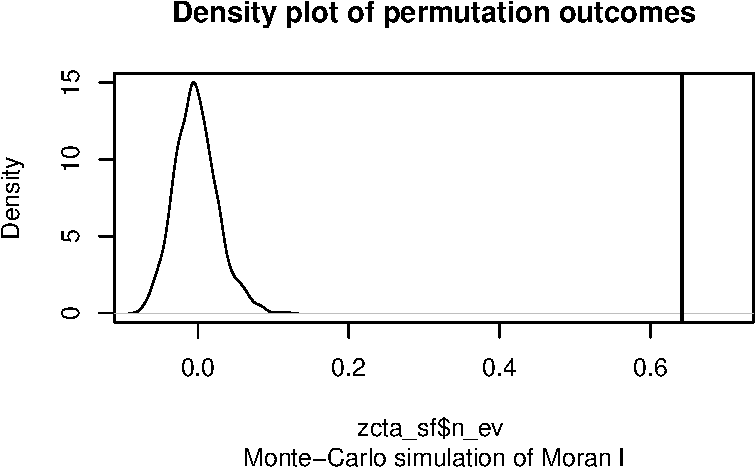
\includegraphics[keepaspectratio]{index_files/figure-pdf/unnamed-chunk-13-1.pdf}}

\textsubscript{Source:
\href{https://h-christy.github.io/24-manuscript/index.qmd.html}{Article
Notebook}}

\subparagraph{Moran's I using Census Tracts as bounding polygons and
Rook definition of
neighbors}\label{morans-i-using-census-tracts-as-bounding-polygons-and-rook-definition-of-neighbors}

\begin{verbatim}
[1] 208002
\end{verbatim}

\textsubscript{Source:
\href{https://h-christy.github.io/24-manuscript/index.qmd.html}{Article
Notebook}}

\textsubscript{Source:
\href{https://h-christy.github.io/24-manuscript/index.qmd.html}{Article
Notebook}}

Moran's I value

\begin{verbatim}
[1] 0.5136527
\end{verbatim}

\textsubscript{Source:
\href{https://h-christy.github.io/24-manuscript/index.qmd.html}{Article
Notebook}}

\subparagraph{visualize neiborhood
relation}\label{visualize-neiborhood-relation}

\textsubscript{Source:
\href{https://h-christy.github.io/24-manuscript/index.qmd.html}{Article
Notebook}}

\begin{verbatim}

    Monte-Carlo simulation of Moran I

data:  ct_sf$n_ev 
weights: ct_listw  
number of simulations + 1: 1000 

statistic = 0.51365, observed rank = 1000, p-value = 0.001
alternative hypothesis: greater
\end{verbatim}

\textsubscript{Source:
\href{https://h-christy.github.io/24-manuscript/index.qmd.html}{Article
Notebook}}

\pandocbounded{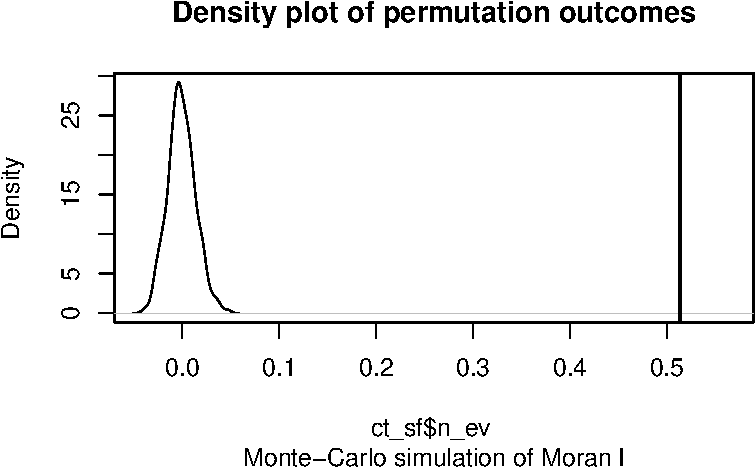
\includegraphics[keepaspectratio]{index_files/figure-pdf/unnamed-chunk-19-1.pdf}}

\textsubscript{Source:
\href{https://h-christy.github.io/24-manuscript/index.qmd.html}{Article
Notebook}}

\paragraph{Local Moran's I: detecting
clusters}\label{local-morans-i-detecting-clusters}

With evidence of clustering globally, we also want information about
where we can find the clusters. In this case, \texttt{spdep::localmoran}
can help use with a Moran's I statistic for each census tract.

\begin{verbatim}
[1] "localmoran" "matrix"     "array"     
\end{verbatim}

\begin{verbatim}
[1] 1784    5
\end{verbatim}

\textsubscript{Source:
\href{https://h-christy.github.io/24-manuscript/index.qmd.html}{Article
Notebook}}

\textsubscript{Source:
\href{https://h-christy.github.io/24-manuscript/index.qmd.html}{Article
Notebook}}

\begin{verbatim}
[1] 1784   26
\end{verbatim}

\begin{verbatim}
    Min.  1st Qu.   Median     Mean  3rd Qu.     Max. 
-2.28334  0.03044  0.19644  0.51365  0.46033 26.79675 
\end{verbatim}

\textsubscript{Source:
\href{https://h-christy.github.io/24-manuscript/index.qmd.html}{Article
Notebook}}

\begin{Shaded}
\begin{Highlighting}[]
\NormalTok{ev\_ct\_local }\OtherTok{\textless{}{-}}\NormalTok{ ct\_sf7 }\SpecialCharTok{|\textgreater{}} \FunctionTok{ggplot}\NormalTok{() }\SpecialCharTok{+}
  \FunctionTok{geom\_sf}\NormalTok{(}\FunctionTok{aes}\NormalTok{(}\AttributeTok{fill=} \FunctionTok{as.numeric}\NormalTok{(local\_i))) }\SpecialCharTok{+}
  \FunctionTok{labs}\NormalTok{(}
    \AttributeTok{title =} \StringTok{"Local moran\textquotesingle{}s I by Census Tracts"}\NormalTok{,}
    \AttributeTok{fill =} \StringTok{"local\_i"}
\NormalTok{  ) }\SpecialCharTok{+}
  \FunctionTok{scale\_fill\_gradient2}\NormalTok{(}\AttributeTok{low=}\StringTok{"darkblue"}\NormalTok{, }\AttributeTok{high=}\StringTok{"red"}\NormalTok{,}
  \AttributeTok{transform =} \StringTok{"pseudo\_log"}\NormalTok{)}
\CommentTok{\# +}
  \FunctionTok{scale\_fill\_viridis\_c}\NormalTok{(}\AttributeTok{na.value =} \StringTok{"gray"}\NormalTok{)}
\CommentTok{\# ggsave(\textquotesingle{}image/ct\_localmoran.png\textquotesingle{}, ev\_ct\_local)}
\NormalTok{ev\_ct\_local}
\end{Highlighting}
\end{Shaded}

\pandocbounded{\includegraphics[keepaspectratio]{image/ct_localmoran.png}}

Local Moran's I significance map

\begin{Shaded}
\begin{Highlighting}[]
\NormalTok{ev\_ct\_local\_p }\OtherTok{\textless{}{-}}\NormalTok{ ct\_sf7 }\SpecialCharTok{|\textgreater{}} \FunctionTok{ggplot}\NormalTok{() }\SpecialCharTok{+}
  \FunctionTok{geom\_sf}\NormalTok{(}\FunctionTok{aes}\NormalTok{(}\AttributeTok{fill=} \FunctionTok{as.numeric}\NormalTok{(local\_p))) }\SpecialCharTok{+}
  \FunctionTok{labs}\NormalTok{(}
    \AttributeTok{title =} \StringTok{"Local moran\textquotesingle{}s I by Census Tracts"}\NormalTok{,}
    \AttributeTok{fill =} \StringTok{"local\_p"}
\NormalTok{  ) }\SpecialCharTok{+}
  \FunctionTok{scale\_fill\_gradient2}\NormalTok{(}\AttributeTok{low=}\StringTok{"darkred"}\NormalTok{, }\AttributeTok{high=}\StringTok{"blue"}\NormalTok{, }\AttributeTok{midpoint=}\FloatTok{0.1}\NormalTok{)}
\CommentTok{\# +}
  \FunctionTok{scale\_fill\_viridis\_c}\NormalTok{(}\AttributeTok{na.value =} \StringTok{"gray"}\NormalTok{)}
\CommentTok{\# ggsave(\textquotesingle{}image/ct\_localmoran\_p.png\textquotesingle{}, ev\_ct\_local\_p)}
\NormalTok{ev\_ct\_local\_p}
\end{Highlighting}
\end{Shaded}

\pandocbounded{\includegraphics[keepaspectratio]{image/ct_localmoran_p.png}}

\subparagraph{local moran permutation
test}\label{local-moran-permutation-test}

\begin{verbatim}
[1] "localmoran" "matrix"     "array"     
\end{verbatim}

\begin{verbatim}
[1] 1784    9
\end{verbatim}

\textsubscript{Source:
\href{https://h-christy.github.io/24-manuscript/index.qmd.html}{Article
Notebook}}

\begin{verbatim}
           Ii          E.Ii       Var.Ii       Z.Ii Pr(z != E(Ii))
1 -0.19651842 -0.0031906570 6.079843e-02 -0.7840577      0.4330062
2  0.00244076  0.0005481923 6.916542e-05  0.2275657      0.8199839
  Pr(z != E(Ii)) Sim Pr(folded) Sim  Skewness Kurtosis
1              0.406          0.203  2.272828 12.18684
2              0.934          0.467 -2.498880 18.68960
\end{verbatim}

\textsubscript{Source:
\href{https://h-christy.github.io/24-manuscript/index.qmd.html}{Article
Notebook}}

From the conditional permutation test, we can plot local significance
map and specify different types of associations. The table below is a
count table for a Moran scatter plot, we can see that among 521 census
tracts with significant pseudo p-values 306 census tracts exhibit
Low-Low associations, 205 census tracts for High-High associations.

\begin{verbatim}

  Low-Low  High-Low  Low-High High-High      <NA> 
      306         8        15       205      1250 
\end{verbatim}

\textsubscript{Source:
\href{https://h-christy.github.io/24-manuscript/index.qmd.html}{Article
Notebook}}

\textsubscript{Source:
\href{https://h-christy.github.io/24-manuscript/index.qmd.html}{Article
Notebook}}

LISA Cluster Map

\begin{Shaded}
\begin{Highlighting}[]
\NormalTok{local\_perm\_map }\OtherTok{\textless{}{-}}\NormalTok{ ct\_sf7 }\SpecialCharTok{|\textgreater{}} \FunctionTok{ggplot}\NormalTok{() }\SpecialCharTok{+}
\FunctionTok{geom\_sf}\NormalTok{(}\FunctionTok{aes}\NormalTok{(}\AttributeTok{fill =}\NormalTok{ scatter)) }\SpecialCharTok{+}
\FunctionTok{labs}\NormalTok{(}
  \AttributeTok{title =} \StringTok{"LISA Cluster Map"}\NormalTok{,}
  \AttributeTok{fill =} \StringTok{"locations"}
\NormalTok{) }\SpecialCharTok{+}
\FunctionTok{scale\_fill\_manual}\NormalTok{(}
  \AttributeTok{values =} \FunctionTok{c}\NormalTok{(}
    \StringTok{\textquotesingle{}High{-}High\textquotesingle{}} \OtherTok{=} \StringTok{\textquotesingle{}red\textquotesingle{}}\NormalTok{,}
    \StringTok{\textquotesingle{}High{-}Low\textquotesingle{}} \OtherTok{=} \StringTok{\textquotesingle{}pink\textquotesingle{}}\NormalTok{,}
    \StringTok{\textquotesingle{}Low{-}High\textquotesingle{}} \OtherTok{=} \StringTok{\textquotesingle{}lightblue\textquotesingle{}}\NormalTok{,}
    \StringTok{\textquotesingle{}Low{-}Low\textquotesingle{}} \OtherTok{=} \StringTok{\textquotesingle{}blue\textquotesingle{}}
\NormalTok{  ),}
  \AttributeTok{na.value =} \StringTok{\textquotesingle{}white\textquotesingle{}}
\NormalTok{)}
\NormalTok{local\_perm\_map}
\CommentTok{\# ggsave(\textquotesingle{}image/manu{-}lisa{-}cluster.png\textquotesingle{}, local\_perm\_map)}
\end{Highlighting}
\end{Shaded}

\pandocbounded{\includegraphics[keepaspectratio]{image/manu-lisa-cluster.png}}

Local Moran's I, pseudo p-values from conditional permutation test, and
identification of the association types for the significant census
tracts, take us to a more in depth understanding of our EV point
pattern. Insight into the hotspots and coldspots of EV adoption,
corresponding to High-High census tracts and Low-Low census tracts is
especially helpful because we are inclined to see the hotspots but
ignore the coldspots. The LISA Cluster Map reveals to us the clusters
centered census tracts with low EV population itself and also surrounded
by neighbors with low EV population, this finding is hardly possible to
get if we only have the positive cases, or already EV owning househols
to visualize. One important aspect of interpreting positive spatial
autocorrelation is demonstrated here, we need to think of the bigger
picture of clustering as the contribution of attribute, in our case EV
count similarity and locational similarity, thus, we won't ignore
clusters that have similar low EV counts also have a role to play in
this picture.

\subsection{Hypothesis Testing}\label{hypothesis-testing}

This section attempts to deal with another aspect we need to account for
when acquiring a positive and significant global autocorrelation value
for our point pattern of interest. In our case, we want to evaluate how
the spatial inhomogeneity of the Washington state can explain for our
initial evidence of clustering.

We want to understand the first-order properties of EV adoption pattern
with the awareness of the underlying landscape of the state they have an
effect on the adoption potential of different locations. We can take a
look at our EV population distribution together with the human
population distribution in WA. They appeared to follow very similar
distribution, and we do recognize that the core of the definition of an
urban area is the spatial distribution of population.

Thus, it will be helpful to set aside other characteristics we associate
with the urban label at the time, examine the relationship between the
two populations in WA. We expect a better understanding of this
relationship can guide us to explore to which extent that the EV counts
variations across locations can be explained by the population count
variations, and how population distribution as a explanation can have
different degrees of effectiveness from one region to another.

\begin{Shaded}
\begin{Highlighting}[]
\NormalTok{distribution\_map }\OtherTok{\textless{}{-}} \FunctionTok{ggplot}\NormalTok{() }\SpecialCharTok{+}
  \FunctionTok{geom\_sf}\NormalTok{(}\AttributeTok{data =}\NormalTok{ ct\_sf, }\AttributeTok{fill =} \StringTok{"lightgray"}\NormalTok{, }\AttributeTok{color =} \StringTok{"white"}\NormalTok{, }\AttributeTok{size =} \FloatTok{0.2}\NormalTok{) }\SpecialCharTok{+} 
  \FunctionTok{geom\_sf}\NormalTok{(}
    \AttributeTok{data =}\NormalTok{ ev\_sf,}
    \FunctionTok{aes}\NormalTok{(}\AttributeTok{size =}\NormalTok{ count,}
    \AttributeTok{color =}\NormalTok{ cb\_palette[}\DecValTok{5}\NormalTok{]),}
    \AttributeTok{alpha =} \FloatTok{0.6}\NormalTok{) }\SpecialCharTok{+}
    \FunctionTok{scale\_size\_continuous}\NormalTok{(}\AttributeTok{name =} \StringTok{"EV Registrations"}\NormalTok{, }\AttributeTok{range =} \FunctionTok{c}\NormalTok{(}\FloatTok{0.1}\NormalTok{, }\DecValTok{15}\NormalTok{)) }\SpecialCharTok{+} 
    \FunctionTok{labs}\NormalTok{(}
    \AttributeTok{title =} \StringTok{"Distribution of ZEVs in WA"}\NormalTok{,}
    \AttributeTok{subtitle =} \StringTok{"Cumulative data to October 31, 2024"}\NormalTok{,}
    \AttributeTok{x =} \StringTok{"longitude"}\NormalTok{,}
    \AttributeTok{y =} \StringTok{"latitude"}
\NormalTok{  ) }\SpecialCharTok{+}
  \FunctionTok{theme\_minimal}\NormalTok{() }\SpecialCharTok{+}
  \FunctionTok{theme}\NormalTok{(}
    \AttributeTok{plot.title =} \FunctionTok{element\_text}\NormalTok{(}\AttributeTok{hjust =} \FloatTok{0.5}\NormalTok{, }\AttributeTok{size =} \DecValTok{14}\NormalTok{),}
    \AttributeTok{plot.subtitle =} \FunctionTok{element\_text}\NormalTok{(}\AttributeTok{hjust =} \FloatTok{0.5}\NormalTok{, }\AttributeTok{size =} \DecValTok{11}\NormalTok{)}
\NormalTok{  ) }\SpecialCharTok{+}
  \FunctionTok{guides}\NormalTok{(}\AttributeTok{color =} \StringTok{"none"}\NormalTok{)}

\FunctionTok{ggsave}\NormalTok{(}\StringTok{"image/manu{-}ev{-}distribution.png"}\NormalTok{, }\AttributeTok{plot =}\NormalTok{ distribution\_map)}

\NormalTok{distribution\_map}
\end{Highlighting}
\end{Shaded}

\pandocbounded{\includegraphics[keepaspectratio]{image/manu-ev-distribution.png}}

NASA GPW data provides us a glimpse of disaggregated human population
data, modeling a human population count for each 1 km\^{}2 grid. We can
take it conveniently as a way to make sense of what population point
pattern can look
like.\footnote{Center for International Earth Science Information
  Network - CIESIN - Columbia University (2018). Gridded Population of
  the World, Version 4 (GPWv4): Population Count Adjusted to Match 2015
  Revision of UN WPP Country Totals, Revision 11. Palisades, NY: NASA
  Socioeconomic Data and Applications Center (SEDAC). doi:
  10.7927/H4PN93PB. Accessed December 4, 2024.}(\citeproc{ref-ciesin2018gpw}{International
Earth Science Information Network (CIESIN) - Columbia University 2018})

\texttt{gpw\_raster}

\begin{verbatim}
class      : RasterLayer 
dimensions : 416, 955, 397280  (nrow, ncol, ncell)
resolution : 0.008333333, 0.008333333  (x, y)
extent     : -124.8667, -116.9083, 45.54167, 49.00833  (xmin, xmax, ymin, ymax)
crs        : +proj=longlat +datum=WGS84 +no_defs 
source     : gpw-popcount.tif 
names      : gpw.popcount 
\end{verbatim}

\textsubscript{Source:
\href{https://h-christy.github.io/24-manuscript/index.qmd.html}{Article
Notebook}}

\textsubscript{Source:
\href{https://h-christy.github.io/24-manuscript/index.qmd.html}{Article
Notebook}}

\begin{verbatim}
[1] 304514      2
\end{verbatim}

\textsubscript{Source:
\href{https://h-christy.github.io/24-manuscript/index.qmd.html}{Article
Notebook}}

\begin{verbatim}
    Min.  1st Qu.   Median     Mean  3rd Qu.     Max. 
   0.000    0.000    0.144   24.585    1.504 7425.167 
\end{verbatim}

\textsubscript{Source:
\href{https://h-christy.github.io/24-manuscript/index.qmd.html}{Article
Notebook}}

\begin{Shaded}
\begin{Highlighting}[]
\NormalTok{gpw\_map }\OtherTok{\textless{}{-}}\NormalTok{ popcount\_sf }\SpecialCharTok{|\textgreater{}} \FunctionTok{ggplot}\NormalTok{(}\FunctionTok{aes}\NormalTok{(}\AttributeTok{fill =}\NormalTok{ pop)) }\SpecialCharTok{+}
  \FunctionTok{geom\_sf}\NormalTok{(}\AttributeTok{color =}\NormalTok{ scales}\SpecialCharTok{::}\FunctionTok{alpha}\NormalTok{(}\StringTok{"white"}\NormalTok{,}\DecValTok{0}\NormalTok{)) }\SpecialCharTok{+}
  \FunctionTok{scale\_fill\_viridis\_c}\NormalTok{(}\AttributeTok{trans =} \StringTok{\textquotesingle{}pseudo\_log\textquotesingle{}}\NormalTok{) }\SpecialCharTok{+} 
  \FunctionTok{theme\_minimal}\NormalTok{() }\SpecialCharTok{+}
  \FunctionTok{labs}\NormalTok{(}
    \AttributeTok{title =} \StringTok{"Population Counts in WA"}\NormalTok{,}
    \AttributeTok{subtitle =} \StringTok{\textquotesingle{}GPW V.4 2020{-}07{-}01\textquotesingle{}}\NormalTok{,}
    \AttributeTok{fill =} \StringTok{"Population Count"}
\NormalTok{    ) }\SpecialCharTok{+} 
  \FunctionTok{theme}\NormalTok{(}
    \AttributeTok{plot.title =} \FunctionTok{element\_text}\NormalTok{(}\AttributeTok{hjust=}\FloatTok{0.5}\NormalTok{),}
    \AttributeTok{plot.subtitle =} \FunctionTok{element\_text}\NormalTok{(}\AttributeTok{hjust=}\FloatTok{0.5}\NormalTok{)}
\NormalTok{    )}

\FunctionTok{ggsave}\NormalTok{(}\StringTok{\textquotesingle{}image/manu{-}gpw{-}raster.png\textquotesingle{}}\NormalTok{, }\AttributeTok{plot =}\NormalTok{ gpw\_map)}

\NormalTok{gpw\_map}
\end{Highlighting}
\end{Shaded}

\begin{Shaded}
\begin{Highlighting}[]
\NormalTok{un\_map }\OtherTok{\textless{}{-}}\NormalTok{ popcount\_sf }\SpecialCharTok{|\textgreater{}} \FunctionTok{ggplot}\NormalTok{(}\FunctionTok{aes}\NormalTok{(}\AttributeTok{fill =}\NormalTok{ pop)) }\SpecialCharTok{+}
  \FunctionTok{geom\_sf}\NormalTok{(}\AttributeTok{color =} \ConstantTok{NA}\NormalTok{) }\SpecialCharTok{+} 
  \FunctionTok{scale\_fill\_viridis}\NormalTok{(}\AttributeTok{option =} \StringTok{\textquotesingle{}C\textquotesingle{}}\NormalTok{, }\AttributeTok{trans =} \StringTok{\textquotesingle{}pseudo\_log\textquotesingle{}}\NormalTok{) }\SpecialCharTok{+} 
  \FunctionTok{theme\_minimal}\NormalTok{() }\SpecialCharTok{+}
  \FunctionTok{labs}\NormalTok{(}
    \AttributeTok{title =} \StringTok{\textquotesingle{}Population Count\textquotesingle{}}\NormalTok{,}
    \AttributeTok{subtitle =} \StringTok{\textquotesingle{}GPW V.4 2020{-}07{-}01\textquotesingle{}}\NormalTok{,}
    \AttributeTok{fill =} \StringTok{\textquotesingle{}Population Count\textquotesingle{}}
\NormalTok{    )}

\FunctionTok{ggsave}\NormalTok{(}\StringTok{\textquotesingle{}image/manu{-}gpw{-}0701.png\textquotesingle{}}\NormalTok{, }\AttributeTok{plot =}\NormalTok{ un\_map)}
\NormalTok{un\_map}
\end{Highlighting}
\end{Shaded}

\pandocbounded{\includegraphics[keepaspectratio]{image/manu-gpw-0701.png}}

Our null hypothesis is: the observed EV point pattern can be directly
explained by the population distribution of WA. In other words, people
in WA have equal chance to adopt EV regardless of where they live, rural
or urban and also regardless of whether their neighbors own EVs or not.

\subsubsection{First order properties of point
process}\label{first-order-properties-of-point-process}

\paragraph{Intensity Function}\label{intensity-function}

One important limitation of this analysis that needs to be addressed is
that we use the WA state boundaries as our observation window. The
drawback of this choice is quite obvious: among the three major
metropolitan areas in WA, two are situated at the borders of the state
-- one with Oregon and the other with Idaho. This can lead to
underestimations, as they can have less neighbors as the result of this
bounding box.

Intensity function we are interested here is the count of event: count
of EVs and count of people in an area

Constructing the \texttt{ppp} object for estimating EV population
intensity is a more straightforward one, we use the 548 distinct points
and marked them with EV registration counts. When it comes to finding an
appropriate way to estimate human population intensity, since ZCTAs are
not a typical statistical division of US Census Bureau, thus, one way to
approach this problem is to use the data of population counts by census
tract and use the centroids of the census tracts to construct
\texttt{ppp} object. Another way we explored is to take the 605
centroids of ZCTAs and request points estimate of population counts also
from NASA APPEEARs.(\citeproc{ref-ciesin2018gpw}{International Earth
Science Information Network (CIESIN) - Columbia University 2018})

With these ppps at hand \texttt{spatstat::density()} can handle these
marked ppp and estimate us the intensity function accounting the marks
as weights.

\subparagraph{\texorpdfstring{\texttt{zev\_ppp}}{zev\_ppp}}\label{zev_ppp}

\textsubscript{Source:
\href{https://h-christy.github.io/24-manuscript/index.qmd.html}{Article
Notebook}}

\textsubscript{Source:
\href{https://h-christy.github.io/24-manuscript/index.qmd.html}{Article
Notebook}}

\textsubscript{Source:
\href{https://h-christy.github.io/24-manuscript/index.qmd.html}{Article
Notebook}}

\pandocbounded{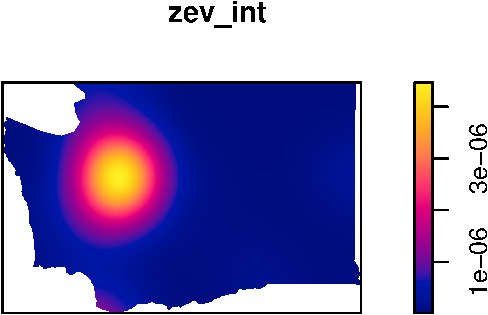
\includegraphics[keepaspectratio]{index_files/figure-pdf/unnamed-chunk-34-1.pdf}}

\textsubscript{Source:
\href{https://h-christy.github.io/24-manuscript/index.qmd.html}{Article
Notebook}}

\begin{verbatim}
[1] 70971.96
\end{verbatim}

\begin{verbatim}
[1] 1.490786e-07
\end{verbatim}

\textsubscript{Source:
\href{https://h-christy.github.io/24-manuscript/index.qmd.html}{Article
Notebook}}

\subparagraph{\texorpdfstring{\texttt{pop\_int}}{pop\_int}}\label{pop_int}

\textsubscript{Source:
\href{https://h-christy.github.io/24-manuscript/index.qmd.html}{Article
Notebook}}

\begin{verbatim}
[1] 7705281
\end{verbatim}

\textsubscript{Source:
\href{https://h-christy.github.io/24-manuscript/index.qmd.html}{Article
Notebook}}

\pandocbounded{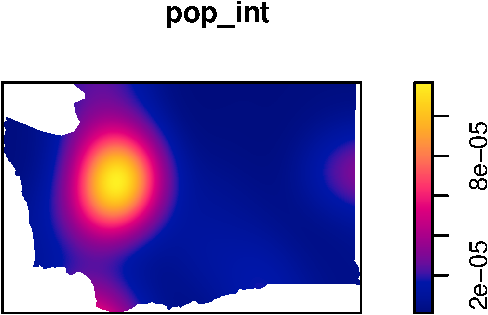
\includegraphics[keepaspectratio]{index_files/figure-pdf/unnamed-chunk-38-1.pdf}}

\textsubscript{Source:
\href{https://h-christy.github.io/24-manuscript/index.qmd.html}{Article
Notebook}}

\begin{Shaded}
\begin{Highlighting}[]
\CommentTok{\# png(\textquotesingle{}image/manu{-}ct{-}ratio.png\textquotesingle{}, width = 750, height = 500)}
\FunctionTok{relative\_int}\NormalTok{(zev\_ppp, pop\_ppp)}
\CommentTok{\# dev.off()}
\end{Highlighting}
\end{Shaded}

\pandocbounded{\includegraphics[keepaspectratio]{image/manu-ct-ratio.png}}

With these ppps at hand \texttt{spatstat::density()} can handle these
marked ppp and estimate us the intensity function accounting the marks
as weights.

\subparagraph{\texorpdfstring{\texttt{gpw\_ppp}}{gpw\_ppp}}\label{gpw_ppp}

\textsubscript{Source:
\href{https://h-christy.github.io/24-manuscript/index.qmd.html}{Article
Notebook}}

\textsubscript{Source:
\href{https://h-christy.github.io/24-manuscript/index.qmd.html}{Article
Notebook}}

\textsubscript{Source:
\href{https://h-christy.github.io/24-manuscript/index.qmd.html}{Article
Notebook}}

\pandocbounded{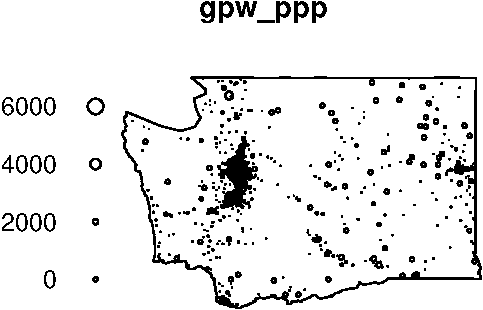
\includegraphics[keepaspectratio]{index_files/figure-pdf/unnamed-chunk-42-1.pdf}}

\textsubscript{Source:
\href{https://h-christy.github.io/24-manuscript/index.qmd.html}{Article
Notebook}}

\begin{verbatim}
[1] 308385.8
\end{verbatim}

\textsubscript{Source:
\href{https://h-christy.github.io/24-manuscript/index.qmd.html}{Article
Notebook}}

\pandocbounded{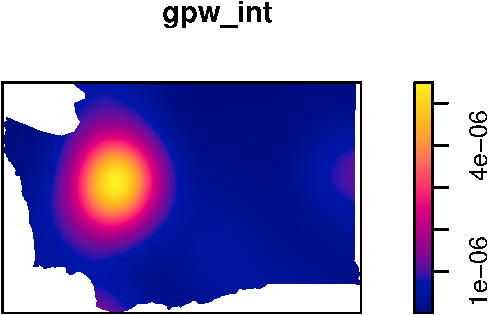
\includegraphics[keepaspectratio]{index_files/figure-pdf/unnamed-chunk-44-1.pdf}}

\textsubscript{Source:
\href{https://h-christy.github.io/24-manuscript/index.qmd.html}{Article
Notebook}}

\begin{Shaded}
\begin{Highlighting}[]
\CommentTok{\# png(\textquotesingle{}image/manu{-}zpts{-}ratio.png\textquotesingle{}, width = 750, height = 500)}
\FunctionTok{relative\_int}\NormalTok{(zev\_ppp, gpw\_ppp)}
\CommentTok{\# dev.off()}
\end{Highlighting}
\end{Shaded}

\pandocbounded{\includegraphics[keepaspectratio]{image/manu-zpts-ratio.png}}

\paragraph{Relative Intensity Surface}\label{relative-intensity-surface}

We use the optimal bandwidths given by spatstat and make adjustments to
calculate intensity ratios between our case point pattern to the base
rate point pattern. By eliminating the effect of the human population
intensity of WA, the relative intensity surface plots still exhibit
uneven ratio from location to location suggesting us that point pattern
of EV population is a special one.\footnote{the interpretation of the
  ratio values have things to do with the different number of points
  between ppp objects, but the color variances is interpretable}

\paragraph{Monte Carlo Simulation}\label{monte-carlo-simulation}

We deploy quadrat count to understand how intensity varies from dividing
the state in to equal regions of ``Low'', ``Medium'' and ``High''
population. Two intensity functions constructed by Census tract level
population count and GPW population count are used as the null point
process in the Monte Carlo simulation.

\subparagraph{divide regions for quadrat
count}\label{divide-regions-for-quadrat-count}

\pandocbounded{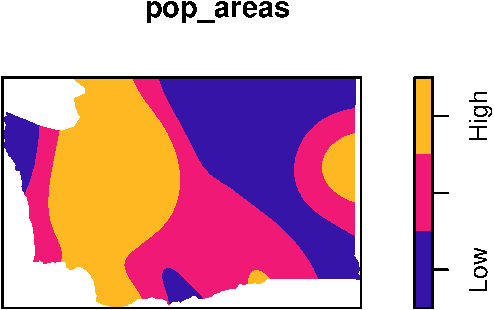
\includegraphics[keepaspectratio]{index_files/figure-pdf/unnamed-chunk-45-1.pdf}}

\textsubscript{Source:
\href{https://h-christy.github.io/24-manuscript/index.qmd.html}{Article
Notebook}}

\subparagraph{computational approach: 999
simulations}\label{computational-approach-999-simulations}

\begin{Shaded}
\begin{Highlighting}[]
\FunctionTok{set.seed}\NormalTok{(}\DecValTok{6805}\NormalTok{)}
\NormalTok{gen\_sims\_ppp }\OtherTok{\textless{}{-}} \ControlFlowTok{function}\NormalTok{(}\AttributeTok{num\_sims =} \DecValTok{999}\NormalTok{) \{}
\NormalTok{  ev\_sims }\OtherTok{\textless{}{-}}\NormalTok{ spatstat.random}\SpecialCharTok{::}\FunctionTok{rpoint}\NormalTok{(}
    \AttributeTok{n =} \FunctionTok{nrow}\NormalTok{(ev\_sf),}
    \AttributeTok{f =}\NormalTok{ pop\_int,}
    \AttributeTok{nsim =}\NormalTok{ num\_sims}
\NormalTok{    )}
  \FunctionTok{return}\NormalTok{(ev\_sims)}
\NormalTok{\}}
\NormalTok{n\_sims }\OtherTok{\textless{}{-}} \DecValTok{999}
\NormalTok{ev\_sims\_list }\OtherTok{\textless{}{-}} \FunctionTok{gen\_sims\_ppp}\NormalTok{()}
\end{Highlighting}
\end{Shaded}

\textsubscript{Source:
\href{https://h-christy.github.io/24-manuscript/index.qmd.html}{Article
Notebook}}

\subparagraph{calculate test statistic from
observations}\label{calculate-test-statistic-from-observations}

\begin{verbatim}
   Low Medium   High 
  1644   9001 197357 
\end{verbatim}

\textsubscript{Source:
\href{https://h-christy.github.io/24-manuscript/index.qmd.html}{Article
Notebook}}

\subparagraph{calculate test statistic from
simulations}\label{calculate-test-statistic-from-simulations}

\begin{Shaded}
\begin{Highlighting}[]
\NormalTok{sims\_region\_counts }\OtherTok{\textless{}{-}} \FunctionTok{lapply}\NormalTok{(}
  \AttributeTok{X =}\NormalTok{ ev\_sims\_list,}
  \AttributeTok{FUN =}\NormalTok{ compute\_quadrat\_counts}
\NormalTok{)}
\NormalTok{sim\_counts\_df }\OtherTok{\textless{}{-}} \FunctionTok{as\_tibble}\NormalTok{(sims\_region\_counts) }\SpecialCharTok{|\textgreater{}} \FunctionTok{t}\NormalTok{() }\SpecialCharTok{|\textgreater{}} \FunctionTok{as\_tibble}\NormalTok{()}
\FunctionTok{colnames}\NormalTok{(sim\_counts\_df) }\OtherTok{\textless{}{-}}\NormalTok{ region\_labels}
\NormalTok{sim\_counts\_df }\SpecialCharTok{|\textgreater{}} \FunctionTok{head}\NormalTok{(}\DecValTok{4}\NormalTok{)}
\end{Highlighting}
\end{Shaded}

\begin{Shaded}
\begin{Highlighting}[]
\NormalTok{bind\_df }\OtherTok{\textless{}{-}} \FunctionTok{bind\_rows}\NormalTok{(sim\_counts\_df, obs\_counts)}
\NormalTok{bind\_df }\SpecialCharTok{|\textgreater{}} \FunctionTok{dim}\NormalTok{()}
\NormalTok{bind\_df }\SpecialCharTok{|\textgreater{}} \FunctionTok{write\_csv}\NormalTok{(}\StringTok{\textquotesingle{}data/manu{-}simulations.csv\textquotesingle{}}\NormalTok{)}
\end{Highlighting}
\end{Shaded}

\textsubscript{Source:
\href{https://h-christy.github.io/24-manuscript/index.qmd.html}{Article
Notebook}}

\pandocbounded{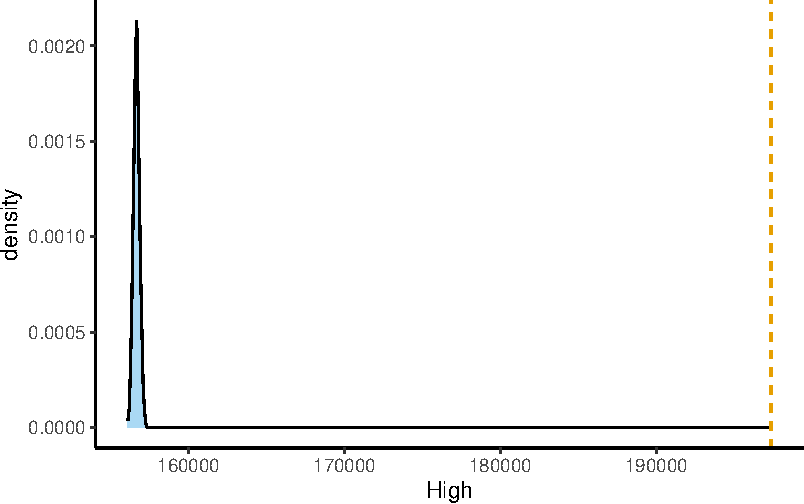
\includegraphics[keepaspectratio]{index_files/figure-pdf/unnamed-chunk-49-1.pdf}}

\textsubscript{Source:
\href{https://h-christy.github.io/24-manuscript/index.qmd.html}{Article
Notebook}}

\begin{Shaded}
\begin{Highlighting}[]
\NormalTok{mc\_sim }\OtherTok{\textless{}{-}} \ControlFlowTok{function}\NormalTok{(im,fpath1, fpath2, }\AttributeTok{num\_sims =} \DecValTok{999}\NormalTok{)\{}
\NormalTok{  n\_regions }\OtherTok{\textless{}{-}} \DecValTok{3}
\NormalTok{  region\_labels }\OtherTok{\textless{}{-}} \FunctionTok{c}\NormalTok{(}\StringTok{"Low"}\NormalTok{, }\StringTok{"Medium"}\NormalTok{, }\StringTok{"High"}\NormalTok{)}
\NormalTok{  int\_vals }\OtherTok{\textless{}{-}}\NormalTok{ im}
\NormalTok{  int\_quant }\OtherTok{\textless{}{-}} \FunctionTok{quantile}\NormalTok{(int\_vals,}\AttributeTok{probs =}\NormalTok{ ((}\DecValTok{0}\SpecialCharTok{:}\NormalTok{n\_regions) }\SpecialCharTok{/}\NormalTok{ n\_regions), }\AttributeTok{na.rm =} \ConstantTok{TRUE}\NormalTok{)}
\NormalTok{  int\_cut }\OtherTok{\textless{}{-}} \FunctionTok{cut}\NormalTok{(int\_vals, }\AttributeTok{breaks =}\NormalTok{ int\_quant, }\AttributeTok{labels =}\NormalTok{ region\_labels)}

\NormalTok{  int\_areas }\OtherTok{\textless{}{-}} \FunctionTok{tess}\NormalTok{(}\AttributeTok{image =}\NormalTok{ int\_cut)}
  \FunctionTok{plot}\NormalTok{(int\_areas)}

  \FunctionTok{set.seed}\NormalTok{(}\DecValTok{6805}\NormalTok{)}
\NormalTok{  gen\_sims\_ppp }\OtherTok{\textless{}{-}} \ControlFlowTok{function}\NormalTok{(num\_sims) \{}
\NormalTok{    spatstat.random}\SpecialCharTok{::}\FunctionTok{rpoint}\NormalTok{(}
      \AttributeTok{n =} \FunctionTok{nrow}\NormalTok{(ev\_sf),}
      \AttributeTok{f =}\NormalTok{ im,}
      \AttributeTok{nsim =}\NormalTok{ num\_sims)}
\NormalTok{  \}}
  
\NormalTok{  sims\_list }\OtherTok{\textless{}{-}} \FunctionTok{gen\_sims\_ppp}\NormalTok{(num\_sims)}

\NormalTok{  compute\_quadrat\_counts }\OtherTok{\textless{}{-}} \ControlFlowTok{function}\NormalTok{(sim\_ppp) \{}
\NormalTok{    counts }\OtherTok{\textless{}{-}} \FunctionTok{quadratcount}\NormalTok{(sim\_ppp, }\AttributeTok{tess =}\NormalTok{ int\_areas) }\SpecialCharTok{|\textgreater{}} \FunctionTok{as.vector}\NormalTok{()}
    \FunctionTok{names}\NormalTok{(counts) }\OtherTok{\textless{}{-}}\NormalTok{ region\_labels}
    \FunctionTok{return}\NormalTok{(counts)}
\NormalTok{  \}}

\NormalTok{  ev\_ppp }\OtherTok{\textless{}{-}} \FunctionTok{sf\_to\_ppp}\NormalTok{(ev\_sf)}
\NormalTok{  obs }\OtherTok{\textless{}{-}} \FunctionTok{compute\_quadrat\_counts}\NormalTok{(ev\_ppp)}

\NormalTok{  sims\_region\_counts }\OtherTok{\textless{}{-}} \FunctionTok{lapply}\NormalTok{(}
    \AttributeTok{X =}\NormalTok{ ev\_sims\_list,}
    \AttributeTok{FUN =}\NormalTok{ compute\_quadrat\_counts}
\NormalTok{    )}
\NormalTok{  sim\_counts\_df }\OtherTok{\textless{}{-}} \FunctionTok{as\_tibble}\NormalTok{(sims\_region\_counts) }\SpecialCharTok{|\textgreater{}} \FunctionTok{t}\NormalTok{() }\SpecialCharTok{|\textgreater{}} \FunctionTok{as\_tibble}\NormalTok{()}
  \FunctionTok{colnames}\NormalTok{(sim\_counts\_df) }\OtherTok{\textless{}{-}}\NormalTok{ region\_labels}

\NormalTok{  bind\_df }\OtherTok{\textless{}{-}} \FunctionTok{bind\_rows}\NormalTok{(sim\_counts\_df, obs\_counts)}
\NormalTok{  bind\_df }\SpecialCharTok{|\textgreater{}} \FunctionTok{write\_csv}\NormalTok{(fpath1)}

\NormalTok{  sims\_plot }\OtherTok{\textless{}{-}}\NormalTok{ bind\_df }\SpecialCharTok{|\textgreater{}} 
    \FunctionTok{ggplot}\NormalTok{(}\FunctionTok{aes}\NormalTok{(}\AttributeTok{x =}\NormalTok{ High)) }\SpecialCharTok{+}
    \FunctionTok{geom\_density}\NormalTok{(}\AttributeTok{fill =}\NormalTok{ cb\_palette[}\DecValTok{2}\NormalTok{], }\AttributeTok{alpha =} \FloatTok{0.5}\NormalTok{) }\SpecialCharTok{+}
    \FunctionTok{geom\_vline}\NormalTok{(}
      \AttributeTok{xintercept =}\NormalTok{ obs[}\StringTok{\textquotesingle{}High\textquotesingle{}}\NormalTok{],}
      \AttributeTok{linetype =} \StringTok{"dashed"}\NormalTok{,}
      \AttributeTok{color =}\NormalTok{ cb\_palette[}\DecValTok{1}\NormalTok{]}
\NormalTok{      ) }\SpecialCharTok{+} 
    \FunctionTok{theme\_classic}\NormalTok{()}

  \FunctionTok{ggsave}\NormalTok{(fpath2, }\AttributeTok{plot =}\NormalTok{ sims\_plot, }\AttributeTok{width =} \DecValTok{14}\NormalTok{, }\AttributeTok{height =} \DecValTok{6}\NormalTok{)}
  
  \FunctionTok{return}\NormalTok{(sims\_plot)}
\NormalTok{\}}
\end{Highlighting}
\end{Shaded}

\begin{Shaded}
\begin{Highlighting}[]
\FunctionTok{mc\_sim}\NormalTok{(gpw\_int, }\StringTok{\textquotesingle{}data/gpw{-}sims.csv\textquotesingle{}}\NormalTok{, }\StringTok{\textquotesingle{}image/gpw{-}distribution.png\textquotesingle{}}\NormalTok{)}
\end{Highlighting}
\end{Shaded}

\pandocbounded{\includegraphics[keepaspectratio]{image/gpw-distribution.png}}

The computational approach gives us an entire distribution of our
statistics of interest, under the simulations of distributing 208002 EV
registrations by human population point process. Given that the observed
value lies on the far right tail of the distribution, the likelihood for
us to observe 197,900 EV registrations in high population regions is a
very low one. Therefore, we can believe that the null hypothesis is not
likely to stand.

The significance of our observed statistics in high population areas is
more like a general picture that justifies our attentions to the spatial
phenomenon of EVs, however, the findings from LISA Cluster Map from the
relative intensity ratio do ask us to pay attention to local differences
and how these local differences can contribute to the characteristics of
the whole point pattern.

\subsection{Discussion}\label{discussion}

With the evidence of clustering and after extracting the effect of
population intensity, we have evidence to describe EV population point
pattern in WA as a whole spatially clustering, and to think about the
implications of this overall unevenness. At the same time, the local
perspective offers insights into the relationship between attributes and
locations in significant clusters.

Knowing the adoption pattern and characteristics of those who already
owns an EV might be a way of analyzing the issue of electric vehicle, if
the aim of the issue is to anticipate a wider adoption and to eliminate
the inequality, getting the glimpse of Low-Low clusters in many ways can
be even more insightful. Another way to think of this issue is that of
EV owning households today assumingly already have a positive view on EV
and they made the decision of buying an EV rationally after evaluating
their own living circumstances. Thus, to promote a more positive and
decent view on electric vehicles and to prepare a more friendly
environment that can support EV purchases, it is evident that more
efforts should be made for the Low-Low clusters.

\subsection{Conclusion}\label{conclusion}

One perspective confirmed by this project is that, it is actually not
that hard to discover EV hotspots, we can find them generally in the
urban areas or metro areas, though they may have different degrees of
concentration. For example, the heart of Seattle Metro area, census
tracts in King County out-performed both the CRS distribution and
population distribution. In the case of Clark county and Spokane city,
the results are less significant, however, may be due to the effect of
the observation window. On the other hand, detecting coldspots requires
many more steps, and we tend to underestimate the contribution of local
Low-Low clusters to the global clusterness. But coldspots are indeed
part of--and might be the essence of--the inequality behind the uneven
spatial pattern of EV adoption.

Most of the analysis in this project is at the exploratory stage. As the
last section of the project, we are to think about where the EDA result
can take us.

Two of the main reason that people usually give for not considering an
EV are: EVs are not affordable, and that EVs are not reliable in terms
of the lack of access to charging equipment.
(\citeproc{ref-kikuchi310Americans2024}{Kikuchi 2024})

Income and charging station accessibility, at a glance are both
following spatial distributions similar toEV population and urban-rural
divisions. Research on EVs has devoted much efforts carrying out the
message that, with possible rebates to make the upfront cost of
purchasing an EV less burdensome, EVs can, in the long term, save
commuters more money than petro and diesel cars. As for the range
anxiety, which is more expressed by potential EV owners than by actual
EV owners, it is explained by that most recent EV owners charge their
vehicles at home on daily bases. This implies that they have private
parking spaces, can afford to install home charging equipment, and the
electric range of their EVs is just sufficient for their daily commute
distances. (\citeproc{ref-AlternativeFuelsDatag}{{``Alternative {Fuels
Data Center}: {Charging Electric Vehicles} at {Home}''} n.d.})

But these facts of today are not there to convince us that affordability
and public charging infrastructure don't really matter much in the
decision of buying an EV. Instead, they can lead us to see that the
diffusion of EVs at a stage where barriers between owners and potential
owners are not only material but also in knowledge.

Looking forward to the 2030 ZEV mandate, all newly sold vehicles
electric, one solution is to make the most of EV charging station. An
analysis by Pew Research Center offers an interesting way to think about
public charging
stations.(\citeproc{ref-shahElectricVehicleCharging2024}{Shah 2024}) Or,
people need to see charging stations for they to develop confidence in
EV before they really use them or even before people actually own an EV.

Addressing the unevenness of adoption and the importance of the
visibility of EV charging station in the EV diffusion process, can be
seen in how Induction Reduction Act incentives target EV charging
stations in rural areas, and in reseach exploring models to determine
the optimal locations for EV charging station installations.
(\citeproc{ref-trancik16potential}{Needell et al. 2016})

The following note is an attempt to take the previous approaches, but
this time analyzing the distribution of EV charging station. Some early
findings from the relative intensity ratio of charging stations on EV
registrations are that the charging station distribution is somewhat
more even compared to the EV registrations.

\begin{tcolorbox}[enhanced jigsaw, colframe=quarto-callout-note-color-frame, toprule=.15mm, arc=.35mm, breakable, leftrule=.75mm, bottomrule=.15mm, colback=white, rightrule=.15mm, left=2mm, opacityback=0]
\begin{minipage}[t]{5.5mm}
\textcolor{quarto-callout-note-color}{\faInfo}
\end{minipage}%
\begin{minipage}[t]{\textwidth - 5.5mm}

\vspace{-3mm}\textbf{Distribution of Public Charging Stations in WA}\vspace{3mm}

\begin{Shaded}
\begin{Highlighting}[]
\ImportTok{import}\NormalTok{ requests}

\NormalTok{api\_key }\OperatorTok{=}\NormalTok{ AFDCKEY}

\NormalTok{url }\OperatorTok{=} \SpecialStringTok{f\textquotesingle{}https://developer.nrel.gov/api/alt{-}fuel{-}stations/v1.csv?api\_key=}\SpecialCharTok{\{}\NormalTok{api\_key}\SpecialCharTok{\}}\SpecialStringTok{\&fuel\_type=ELEC\&state=WA\&access=public\textquotesingle{}}
\NormalTok{output\_file }\OperatorTok{=} \StringTok{\textquotesingle{}data/ev\_charging\_stations\_wa.csv\textquotesingle{}}
\NormalTok{response }\OperatorTok{=}\NormalTok{ requests.get(url)}
\ControlFlowTok{if}\NormalTok{ response.status\_code }\OperatorTok{==} \DecValTok{200}\NormalTok{:}
    \ControlFlowTok{with} \BuiltInTok{open}\NormalTok{(output\_file, }\StringTok{\textquotesingle{}wb\textquotesingle{}}\NormalTok{) }\ImportTok{as}\NormalTok{ f:}
\NormalTok{        f.write(response.content)}
    \BuiltInTok{print}\NormalTok{(}\SpecialStringTok{f"}\SpecialCharTok{\{}\NormalTok{output\_file}\SpecialCharTok{\}}\SpecialStringTok{"}\NormalTok{)}
\ControlFlowTok{else}\NormalTok{:}
    \BuiltInTok{print}\NormalTok{(}\SpecialStringTok{f"status code }\SpecialCharTok{\{}\NormalTok{response}\SpecialCharTok{.}\NormalTok{status\_code}\SpecialCharTok{\}}\SpecialStringTok{: }\SpecialCharTok{\{}\NormalTok{response}\SpecialCharTok{.}\NormalTok{text}\SpecialCharTok{\}}\SpecialStringTok{"}\NormalTok{)}
\end{Highlighting}
\end{Shaded}

\textsubscript{Source:
\href{https://h-christy.github.io/24-manuscript/index.qmd.html}{Article
Notebook}}

\textsubscript{Source:
\href{https://h-christy.github.io/24-manuscript/index.qmd.html}{Article
Notebook}}

\textsubscript{Source:
\href{https://h-christy.github.io/24-manuscript/index.qmd.html}{Article
Notebook}}

\pandocbounded{\includegraphics[keepaspectratio]{image/manu-urb-stations.png}}

\textsubscript{Source:
\href{https://h-christy.github.io/24-manuscript/index.qmd.html}{Article
Notebook}}

\begin{verbatim}
Reading layer `evse' from data source `/Users/toyuan/24-manuscript/data/evse.gpkg' using driver `GPKG'
Simple feature collection with 2662 features and 6 fields
Geometry type: POINT
Dimension:     XY
Bounding box:  xmin: -124.6629 ymin: 45.56257 xmax: -117.0435 ymax: 48.99526
Geodetic CRS:  WGS 84
\end{verbatim}

\begin{verbatim}
            geom          count      
 POINT        :2647   Min.   :1.000  
 epsg:4326    :   0   1st Qu.:1.000  
 +proj=long...:   0   Median :1.000  
                      Mean   :1.006  
                      3rd Qu.:1.000  
                      Max.   :2.000  
\end{verbatim}

\textsubscript{Source:
\href{https://h-christy.github.io/24-manuscript/index.qmd.html}{Article
Notebook}}

\begin{Shaded}
\begin{Highlighting}[]
\NormalTok{urb\_station\_map }\OtherTok{\textless{}{-}} \FunctionTok{ggplot}\NormalTok{() }\SpecialCharTok{+}
  \FunctionTok{geom\_sf}\NormalTok{(}\AttributeTok{data =}\NormalTok{ ct\_sf, }\AttributeTok{fill =} \StringTok{"lightgray"}\NormalTok{, }\AttributeTok{color =} \StringTok{"white"}\NormalTok{, }\AttributeTok{size =} \FloatTok{0.2}\NormalTok{) }\SpecialCharTok{+} 
  \FunctionTok{geom\_sf}\NormalTok{(}\AttributeTok{data =}\NormalTok{ wa\_stations\_sf, }\AttributeTok{color =}\NormalTok{ cb\_palette[}\DecValTok{3}\NormalTok{], }\AttributeTok{alpha =} \FloatTok{0.6}\NormalTok{) }\SpecialCharTok{+}
  \FunctionTok{geom\_sf}\NormalTok{(}\AttributeTok{data =} \FunctionTok{to\_4326}\NormalTok{(urban\_poly), }\FunctionTok{aes}\NormalTok{(}\AttributeTok{fill =} \StringTok{"Urban Areas"}\NormalTok{), }\AttributeTok{color =} \StringTok{"pink"}\NormalTok{, }\AttributeTok{alpha =} \FloatTok{0.3}\NormalTok{) }\SpecialCharTok{+}
  \FunctionTok{scale\_fill\_manual}\NormalTok{(}\AttributeTok{name =} \StringTok{"Legend"}\NormalTok{, }\AttributeTok{values =} \FunctionTok{c}\NormalTok{(}\StringTok{"Urban Areas"} \OtherTok{=} \StringTok{"pink"}\NormalTok{)) }\SpecialCharTok{+}
  \FunctionTok{labs}\NormalTok{(}
    \AttributeTok{title =} \StringTok{"Distribution of Public EV Charging Stations in WA"}\NormalTok{,}
    \AttributeTok{subtitle =} \StringTok{"urban areas"}
\NormalTok{  ) }\SpecialCharTok{+}
  \FunctionTok{theme\_minimal}\NormalTok{() }\SpecialCharTok{+}
  \FunctionTok{theme}\NormalTok{(}
    \AttributeTok{plot.title =} \FunctionTok{element\_text}\NormalTok{(}\AttributeTok{hjust =} \FloatTok{0.5}\NormalTok{, }\AttributeTok{size =} \DecValTok{16}\NormalTok{),}
    \AttributeTok{plot.subtitle =} \FunctionTok{element\_text}\NormalTok{(}\AttributeTok{hjust =} \FloatTok{0.5}\NormalTok{, }\AttributeTok{size =} \DecValTok{12}\NormalTok{)}
\NormalTok{  )}

\FunctionTok{ggsave}\NormalTok{(}\StringTok{"image/manu{-}urb{-}stations.png"}\NormalTok{, }\AttributeTok{plot =}\NormalTok{ urb\_station\_map)}
\NormalTok{urb\_station\_map}
\CommentTok{\# 4326}
\end{Highlighting}
\end{Shaded}

\pandocbounded{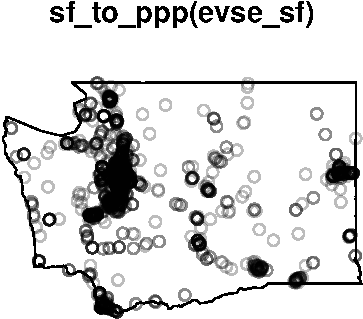
\includegraphics[keepaspectratio]{index_files/figure-pdf/unnamed-chunk-55-1.pdf}}

\textsubscript{Source:
\href{https://h-christy.github.io/24-manuscript/index.qmd.html}{Article
Notebook}}

\texttt{station\_ppp}

\textsubscript{Source:
\href{https://h-christy.github.io/24-manuscript/index.qmd.html}{Article
Notebook}}

\begin{verbatim}
[1] 2647
\end{verbatim}

\textsubscript{Source:
\href{https://h-christy.github.io/24-manuscript/index.qmd.html}{Article
Notebook}}

\pandocbounded{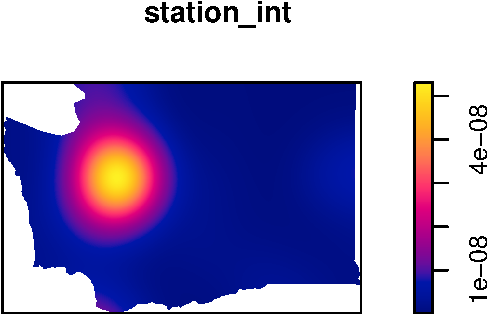
\includegraphics[keepaspectratio]{index_files/figure-pdf/unnamed-chunk-58-1.pdf}}

\textsubscript{Source:
\href{https://h-christy.github.io/24-manuscript/index.qmd.html}{Article
Notebook}}

\begin{Shaded}
\begin{Highlighting}[]
\FunctionTok{png}\NormalTok{(}\StringTok{\textquotesingle{}image/manu{-}station{-}ratio.png\textquotesingle{}}\NormalTok{, }\AttributeTok{width =} \DecValTok{750}\NormalTok{, }\AttributeTok{height =} \DecValTok{500}\NormalTok{)}
\FunctionTok{relative\_int}\NormalTok{(station\_ppp, zev\_ppp)}
\FunctionTok{dev.off}\NormalTok{()}
\end{Highlighting}
\end{Shaded}

\pandocbounded{\includegraphics[keepaspectratio]{image/manu-station-ratio.png}}

\pandocbounded{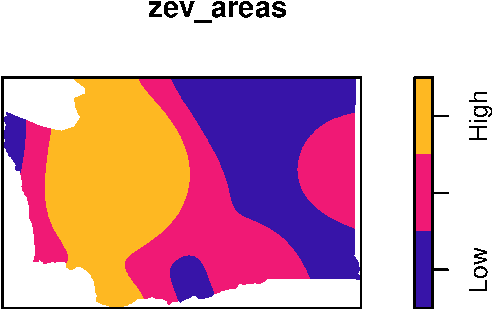
\includegraphics[keepaspectratio]{index_files/figure-pdf/unnamed-chunk-59-1.pdf}}

\textsubscript{Source:
\href{https://h-christy.github.io/24-manuscript/index.qmd.html}{Article
Notebook}}

\begin{Shaded}
\begin{Highlighting}[]
\FunctionTok{set.seed}\NormalTok{(}\DecValTok{6805}\NormalTok{)}
\NormalTok{evse\_sims\_ppp }\OtherTok{\textless{}{-}} \ControlFlowTok{function}\NormalTok{(}\AttributeTok{num\_sims =} \DecValTok{999}\NormalTok{) \{}
\NormalTok{  evse\_sims }\OtherTok{\textless{}{-}}\NormalTok{ spatstat.random}\SpecialCharTok{::}\FunctionTok{rpoint}\NormalTok{(}
    \AttributeTok{n =} \FunctionTok{nrow}\NormalTok{(evse\_sf),}
    \AttributeTok{f =}\NormalTok{ zev\_int,}
    \AttributeTok{nsim =}\NormalTok{ num\_sims}
\NormalTok{    )}
  \FunctionTok{return}\NormalTok{(evse\_sims)}
\NormalTok{\}}
\NormalTok{n\_sims }\OtherTok{\textless{}{-}} \DecValTok{999}
\NormalTok{evse\_sims\_list }\OtherTok{\textless{}{-}} \FunctionTok{evse\_sims\_ppp}\NormalTok{()}
\end{Highlighting}
\end{Shaded}

\begin{Shaded}
\begin{Highlighting}[]
\NormalTok{compute\_quadrat\_counts2 }\OtherTok{\textless{}{-}} \ControlFlowTok{function}\NormalTok{(sim\_ppp) \{}
\NormalTok{  counts }\OtherTok{\textless{}{-}} \FunctionTok{quadratcount}\NormalTok{(sim\_ppp, }\AttributeTok{tess =}\NormalTok{ zev\_areas) }\SpecialCharTok{|\textgreater{}} \FunctionTok{as.vector}\NormalTok{()}
  \FunctionTok{names}\NormalTok{(counts) }\OtherTok{\textless{}{-}}\NormalTok{ region\_labels}

  \FunctionTok{return}\NormalTok{(counts)}
\NormalTok{\}}
\end{Highlighting}
\end{Shaded}

\begin{Shaded}
\begin{Highlighting}[]
\NormalTok{obs\_evse }\OtherTok{\textless{}{-}} \FunctionTok{compute\_quadrat\_counts2}\NormalTok{(station\_ppp)}
\NormalTok{obs\_evse}
\end{Highlighting}
\end{Shaded}

\begin{Shaded}
\begin{Highlighting}[]
\NormalTok{sim\_evse\_counts }\OtherTok{\textless{}{-}} \FunctionTok{lapply}\NormalTok{(}
  \AttributeTok{X =}\NormalTok{ evse\_sims\_list,}
  \AttributeTok{FUN =}\NormalTok{ compute\_quadrat\_counts2}
\NormalTok{)}
\NormalTok{sim\_evse\_df }\OtherTok{\textless{}{-}} \FunctionTok{as\_tibble}\NormalTok{(sim\_evse\_counts) }\SpecialCharTok{|\textgreater{}} \FunctionTok{t}\NormalTok{() }\SpecialCharTok{|\textgreater{}} \FunctionTok{as\_tibble}\NormalTok{()}
\FunctionTok{colnames}\NormalTok{(sim\_evse\_df) }\OtherTok{\textless{}{-}}\NormalTok{ region\_labels}
\NormalTok{sim\_evse\_df }\SpecialCharTok{|\textgreater{}} \FunctionTok{head}\NormalTok{(}\DecValTok{4}\NormalTok{)}
\end{Highlighting}
\end{Shaded}

\begin{Shaded}
\begin{Highlighting}[]
\NormalTok{bind\_evse\_df }\OtherTok{\textless{}{-}} \FunctionTok{bind\_rows}\NormalTok{(sim\_evse\_df, obs\_evse)}
\NormalTok{bind\_evse\_df }\SpecialCharTok{|\textgreater{}} \FunctionTok{dim}\NormalTok{()}
\end{Highlighting}
\end{Shaded}

\begin{Shaded}
\begin{Highlighting}[]
\NormalTok{evse\_sim\_plot }\OtherTok{\textless{}{-}}\NormalTok{ bind\_evse\_df }\SpecialCharTok{|\textgreater{}}
  \FunctionTok{ggplot}\NormalTok{(}\FunctionTok{aes}\NormalTok{(}\AttributeTok{x=}\NormalTok{Medium)) }\SpecialCharTok{+} 
  \FunctionTok{geom\_density}\NormalTok{(}\AttributeTok{fill=}\NormalTok{cb\_palette[}\DecValTok{2}\NormalTok{], }\AttributeTok{alpha =} \FloatTok{0.5}\NormalTok{) }\SpecialCharTok{+}
  \FunctionTok{geom\_vline}\NormalTok{(}\AttributeTok{xintercept =}\NormalTok{ obs\_evse[}\StringTok{\textquotesingle{}Medium\textquotesingle{}}\NormalTok{], }\AttributeTok{linetype =} \StringTok{\textquotesingle{}dashed\textquotesingle{}}\NormalTok{, }\AttributeTok{color =}\NormalTok{ cb\_palette[}\DecValTok{1}\NormalTok{]) }\SpecialCharTok{+} 
  \FunctionTok{theme\_classic}\NormalTok{()}

\NormalTok{evse\_sim\_plot}
\FunctionTok{ggsave}\NormalTok{(}\StringTok{\textquotesingle{}image/evse{-}sims{-}plot.png\textquotesingle{}}\NormalTok{, evse\_sim\_plot)}
\end{Highlighting}
\end{Shaded}

\pandocbounded{\includegraphics[keepaspectratio]{image/evse-sims-plot.png}}

\end{minipage}%
\end{tcolorbox}

For the interpretation of the interesting census tracts we find in the
LISA cluster map, there is much to anticipate if domain knowledge of the
state and locals is introduced.

\phantomsection\label{refs}
\begin{CSLReferences}{1}{0}
\bibitem[\citeproctext]{ref-AlternativeFuelsDatag}
{``Alternative {Fuels Data Center}: {Charging Electric Vehicles} at
{Home}.''} n.d. https://afdc.energy.gov/fuels/electricity-charging-home.
Accessed December 1, 2024.

\bibitem[\citeproctext]{ref-bureauMetropolitanMicropolitanStatistical}
Bureau, US Census. n.d. {``Metropolitan and {Micropolitan Statistical
Areas Population Totals}: 2020-2023.''} \emph{Census.gov}.
https://www.census.gov/data/tables/time-series/demo/popest/2020s-total-metro-and-micro-statistical-areas.html.
Accessed December 10, 2024.

\bibitem[\citeproctext]{ref-ElectricVehiclePopulation}
{``Electric {Vehicle Population Data} {\textbar} {Data}.{WA} {\textbar}
{State} of {Washington}.''} 2024.
https://data.wa.gov/Transportation/Electric-Vehicle-Population-Data/f6w7-q2d2/about\_data;
data.wa.gov.

\bibitem[\citeproctext]{ref-ciesin2018gpw}
International Earth Science Information Network (CIESIN) - Columbia
University, Center for. 2018. {``Gridded Population of the World,
Version 4 (GPWv4): Population Count Adjusted to Match 2015 Revision of
UN WPP Country Totals, Revision 11.''} Palisades, NY: NASA Socioeconomic
Data; Applications Center (SEDAC).
\url{https://doi.org/10.7927/H4PN93PB}.

\bibitem[\citeproctext]{ref-kikuchi310Americans2024}
Kikuchi, Alec Tyson and Emma. 2024. {``About 3 in 10 {Americans} Would
Seriously Consider Buying an Electric Vehicle.''} \emph{Pew Research
Center}.
\url{https://www.pewresearch.org/short-reads/2024/06/27/about-3-in-10-americans-would-seriously-consider-buying-an-electric-vehicle/}.

\bibitem[\citeproctext]{ref-trancik16potential}
Needell, Zachary A., James Mcnerney, Michael T. Chang, and Jessika E.
Trancik. 2016. {``Potential for Widespread Electrification of Personal
Vehicle Travel in the United States.''} \emph{Nature Energy} 1 (August):
16112.
\url{https://proxy.library.georgetown.edu/login?url=https://www.proquest.com/scholarly-journals/potential-widespread-electrification-personal/docview/2218221398/se-2}.

\bibitem[\citeproctext]{ref-shahElectricVehicleCharging2024}
Shah, Samuel Bestvater and Sono. 2024. {``Electric {Vehicle Charging
Infrastructure} in the {U}.{S}.''} \emph{Pew Research Center}.
\url{https://www.pewresearch.org/data-labs/2024/05/23/electric-vehicle-charging-infrastructure-in-the-u-s/}.

\end{CSLReferences}




\end{document}
